\section{General Information}
\par{Figbook is an online collaborative writing system that facilitates writing/editing and styling a novel. It allows authors and editors to work on their project collaboratively in a central place.}

\subsection{System Overview}
\par{Figbook allows multiple authors to collaborate on a book online. It allows editors to log in and edit the manuscript and constantly communicate with authors about their project. \\ \\The system aims to provide a platform for different people in the publishing world (authors, editors, proof-readers etc) to come together and complete a project without having to constantly send manuscripts back and forth via email/mail etc.}

\subsection{System Configuration}
\par{Figbook is hosted online. Any users that wish to use it need an Internet connection and a web browser to access the website.\\ \\The website structure is defined in \textbf{HTML} and styled with \textbf{CSS}. Client side validation is done in \textbf{Javascript} and any dynamic creation and content changes are done with \textbf{JQuery}.\\ \\The client (web browser) communicates with a php enabled \textbf{Apache server via Ajax} calls that send through \textbf{JSON} objects. Depending on the request received from the client, the server may communicate with a mySQL server to persist and/or retrieve information. This information is communicated back to the client in a JSON object. Refer to the diagram below for further clarification:}

\begin{figure}[h]
	\centering
	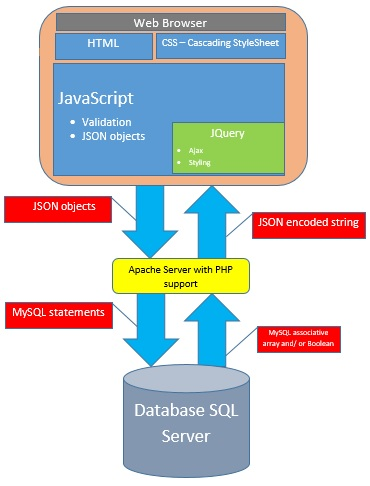
\includegraphics[scale=0.69]{images/webconfig.jpg}
	\caption{Web System Configuration}
\end{figure}

\subsection{User Access Levels}
In order to use the system users have to have an account. There exists a guest account that shows potential users the available services, but they'll need to register an account to use them.

\subsection{Installing}
\par{In order to use this system, users must have a browser with Javascript enabled installed.}
